\newpage
\chapter{METODE PENELITIAN} \label{Bab III}

\section{Alur Penelitian} \label{III.Alur}
Pada penelitian ini, alur dirancang untuk memastikan setiap tahapan pemrosesan dilakukan secara sistematis dan efisien. Alur penelitian ini mencerminkan langkah-langkah utama terkait bagaimana proses yang dilakukan dalam penelitian, dari awal sampai dengan akhir. Gambarkan dalam bentuk diagram alir (\textit{flowchart}) seperti yang terlihat pada Gambar \ref{fig:3.alur}. \par

\begin{figure}[H] % Kalau menggunakan H, posisi gambar akan tepat dibawah teks
    \centering
    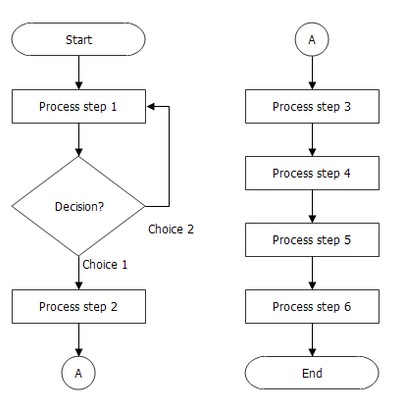
\includegraphics[width=0.6\textwidth]{figure/flowchart.jpg}
    \caption{Alur Penelitian}
    \label{fig:3.alur}
\end{figure}

\section{Penjabaran Langkah Penelitian} \label{III.Jabar Alur}
Jelaskan secara general langkah-langkah alur penelitian, yang sudah tergambar dalam flowchart di subbab \ref{III.Alur}. Subsubbab berikut harus sesuai dengan jumlah entitas langkah pada alur penelitian. \par

\subsection{Langkah 1} \label{III.Langkah 1}
Penjelasan Langkah 1. \par

\subsection{Langkah 2} \label{III.Langkah 2}
Penjelasan Langkah 2. \par

\section{Alat dan Bahan Tugas Akhir} \label{III.Alat dan Bahan}
Berisi alat-alat dan bahan-bahan yang digunakan dalam penelitian. \par

\subsection{Alat} \label{III.Alat}
Alat yang digunakan untuk melakukan penelitian, dapat berupa computer, PC, Arduino, raspberry, etc. Contoh: \par
\begin{enumerate}[noitemsep]
	\item \textit{Notebook} dengan spesifikasi minumum sistem operasi Windows 11, processor AMD Ryzen 5 7430 CPU @ 6 core/2,3 GHz, RAM 16GB DDR4, grafis AMD Radeon RX Vega 7 2GB, SSD 512 GB.
	\item \textit{Smartphone} dengan spesifikasi OS Android OS 12, CPU Snapdragon 778G Octa-core, GPU Adreno 642L, memori 128 GB, RAM 6 GB.
	\item Platform game engine Godot v4.3
	\item Code editor Microsoft Visual Studio Code
	\item Github
\end{enumerate}

\subsection{Bahan} \label{III.Bahan}
Bahan yang digunakan/diperlukan untuk melakukan penelitian, dapat berupa: \par
\begin{enumerate}[noitemsep]
	\item Dataset pihak lain yang diperoleh dengan izin atau dalam lisensi yang diizinkan untuk digunakan secara langsung,
	\item Dataset pihak pertama yang disusun sendiri melalui quisioner, observasi, atau interview,
	\item Dokumen panduan yang mengacu pada standar, hasil tugas akhir, atau artikel yang disitasi dan digunakan. 
\end{enumerate}

\section{Metode Pengembangan} \label{III.Metode}
Membahas mengenai metode yang digunakan dalam penelitian, berdasarkan dasar teori yang sebelumnya sudah dijelaskan pada subbab \ref{II.Teori}. Setiap Tugas Akhir wajib memiliki metode dalam pelaksanaannya yang sesuai dengan penelitian yang dikerjakan: \par
\begin{enumerate}[noitemsep]
	\item Alur pengembangan tugas akhir, menggunakan flowchart
	\item Cara pengumpulan data yang digunakan ()Kuesioner, Wawancara, pengujian, dan lainnya)
	\item Metode pengembangan tugas akhir (Metode Waterfall, Agile, RAD, dan lainnya).
\end{enumerate}
Subbab ini akan berhubungan erat dengan Subbab \ref{IV.Hasil}. \par

\section{Ilustrasi Perhitungan Metode} \label{III.Ilustrasi}
Dalam penelitian ini, hasil perhitungan dari program akan melalui serangkaian pengujian untuk mengevaluasi tingkat keakuratan model yang digunakan. Data dummy tersebut dapat dilihat pada Tabel \ref{table:3.dummy}. \par

\begin{longtable}{|c|c|c|c|c|c|c|c|c|}
	\caption{Data \textit{dummy} Pengujian}
	\label{table:3.dummy}\\
	\hline
	\multirow{2}{*}{\textbf{Subjek}} & \multicolumn{7}{|c|}{\textbf{Hasil Prediksi (BPM)}} & \multirow{2}{*}{\textbf{GT}} \\ \cline{2-8}
    & \textbf{F} & \textbf{NA} & \textbf{NO} & \textbf{RC} & \textbf{LC} & \textbf{M} & \textbf{C} & \\ 
        \hline
	   \endfirsthead
       \hline
       \multirow{2}{*}{\textbf{Subjek}} & \multicolumn{7}{|c|}{\textbf{Hasil Prediksi (BPM)}} & \multirow{2}{*}{\textbf{GT}} \\ \cline{2-8}
    & \textbf{F} & \textbf{NA} & \textbf{NO} & \textbf{RC} & \textbf{LC} & \textbf{M} & \textbf{C} & \\ 
    \hline
	\endhead
	\hline
	\endfoot
	\hline
	\endlastfoot
	1 & 68 & 69 & 68 & 70 & 68 & 71 & 69 & 68 \\ 
	\hline
	2 & 69 & 69 & 68 & 70 & 68 & 71 & 69 & 69 \\
	\hline
	3 & 70 & 70 & 69 & 71 & 68 & 73 & 69 & 70\\
	\hline
	4 & 71 & 70 & 70 & 72 & 69 & 73 & 70 & 71 \\
	\hline
	5 & 72 & 72 & 70 & 72 & 70 & 74 & 70 & 72 \\
	\hline
        6 & 73 & 72 & 71 & 74 & 71 & 76 & 71 & 73 \\ 
	\hline
	7 & 74 & 73 & 72 & 74 & 72 & 77 & 71 & 74 \\
	\hline
	8 & 75 & 74 & 72 & 74 & 73 & 77 & 73 & 75\\
	\hline
	9 & 76 & 75 & 73 & 75 & 74 & 78 & 75 & 76 \\
	\hline
	10 & 77 & 76 & 74 & 78 & 75 & 78 & 76 & 77
\end{longtable}